\documentclass[13pt	]{beamer}
\usepackage{lipsum}
\usepackage{tikz}
\usepackage{verbatim}
\usepackage{graphicx}
\addtobeamertemplate{navigation symbols}{}{%
    \usebeamerfont{footline}%
    \usebeamercolor[fg]{footline}%
    \hspace{1em}%
    \insertframenumber
}
\setbeamercolor{footline}{fg=black}
\setbeamerfont{footline}{series=\bfseries}
 
\usetikzlibrary{calc,trees,positioning,arrows,chains,shapes.geometric,
decorations.pathreplacing,decorations.pathmorphing,shapes,matrix,shapes}
\tikzstyle{decision} = [diamond, draw, fill=blue!20, text width=4.5em, text badly centered, node distance=3cm, inner sep=0pt]
\tikzstyle{block} = [rectangle, draw, fill=blue!20, text width=15em, text centered, rounded corners, minimum height=3em]
\tikzstyle{line} = [draw, -latex']
\tikzstyle{cloud} = [draw, ellipse,fill=red!20, node distance=3cm,minimum height=2em]
\newcommand\Fontvi{\fontsize{6}{7.2}\selectfont}
%\usepackage{beamerthemeBoadilla}
%\usepackage{media9}
\usepackage[labelformat=empty,font=small,format=hang,labelfont=bf,up,textfont=it,up]{caption} 
\title{\large\textsc{Trajectory Of Quadrator Using NMPC}}
\date{Nov 13, 2014}
%\author{} 
%\beamersetuncovermixins{\opaqueness<1>{25}}%{\opaqueness<2->{15}}

\begin{document}

\begin{frame}
\titlepage
\begin{center}

\textsf{\footnotesize Bahador Kocer, Fabian Girribach , Ramin Zohouri}\\
%\textsf{\footnotesize Maren Bennewitz, Martin Riedmiller}\\
%\textsf{\footnotesize Humanoid Robots Lab}\\
\textsf{\footnotesize NOCEO Summer School 2015}\\
\text{\footnotesize University of Freiburg}
%\begin{figure}

%\includegraphics[scale=0.10]{img/Kinect.jpg}
%\end{figure}
\end{center}
\end{frame} 


\begin{frame}
\frametitle{Motivation}
\begin{itemize}
\item Real time control problems
\item Under actuated dynamics
\item Strongly coupled non-linearities
\begin{figure}
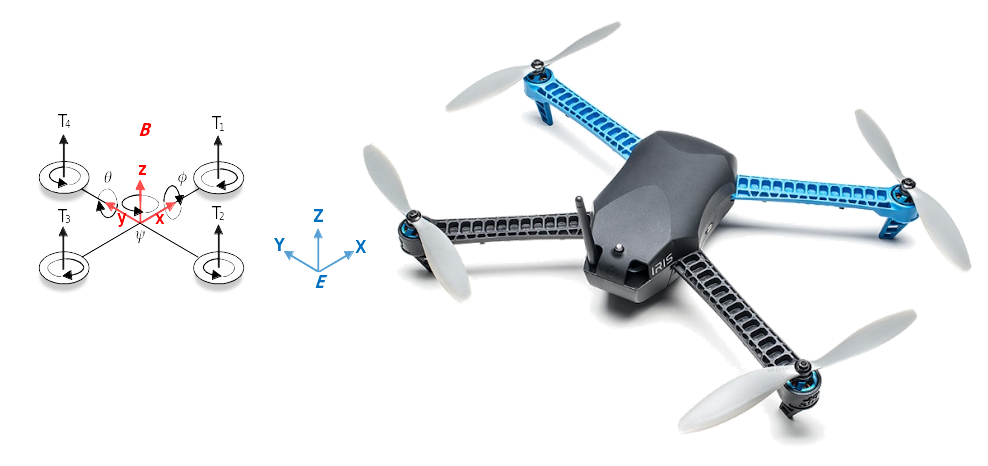
\includegraphics[scale=0.3]{./figures/quad.png}
\caption{\tiny Quadrator by 3D-Robotics.}
\end{figure}
\end{itemize}


\end{frame}

\begin{frame}
\frametitle{Dynamic Model Of Quadcopter} 
\begin{center}
\fontsize{8}{7.2}\selectfont

%\begin{equation} 
%\begin{split}
\begin{align}
&\ddot{\phi}=\dot{\theta}\dot{\psi}a_1 + \dot{\theta}a_2;~~\ddot{\theta}=\dot{\phi}\dot{\psi} a_3 -\dot{\phi}a_4;~~\ddot{\psi}=\dot{\theta}\dot{\phi}a_5+b_3 U_4 \\
&\Omega_r +b_1 U_2;~~\Omega_r +b_2 U_3\\
&\ddot{x}=u_x \frac{1}{m} U_1;~~\ddot{z}=g-\big(cos(\phi)cos(\theta)\big)\frac{1}{m} U_1;~~\ddot{y}=u_y \frac{1}{m}U_1.\\
&a_1=\frac{(I_{yy}-I_{zz})}{I_{xx}};~~a_2=\frac{J_r}{I_{xx}};~~a_3=\frac{(I_{zz}-I_{xx})}{I_{yy}} \\
&a_4=\frac{J_r}{I_{yy}};~~a_5=\frac{(I_{xx}-I_{yy})}{I_{zz}};~~b_1=\frac{l}{I_{xx}}\\
&b_2=\frac{l}{I_{yy}};~~b_3=\frac{l}{I_{zz}};~~b_2=\frac{l}{I_{yy}};~~b_3=\frac{l}{I_{zz}}\\ 
&u_a=cos(\phi)cos(\theta);~~u_x=cos(\phi)sin(\theta)cos(\psi)+sin(\phi)sin(\psi)\\
&u_y=cos(\phi)sin(\theta)cos(\psi)-sin(\phi)cos(\psi)\\
&J_{r}\dot{\theta} \Omega_r the~gyroscopic~effect~due~to~the~propeller\\
&dynamics.~It~is~assumed~that~U_1 = \Omega_r.
\end{align} 
%\end{split}
%\end{equation}
\end{center}
\end{frame}

\begin{frame}
\frametitle{Event Related Potential (ERP) Based Learning}
\begin{table}[h!] 
  \caption{Tricopter Parameters} 
\begin{center} 
\begin{tabular}{|c|c|c|} 
  \hline 
  Paremeter & Value (Unit) \\ 
  \hline
  $Controller$ & $NMPC$ \\ 
   \hline
  $Hessian Approximation$ & $Gauss Newton$ \\ 
   \hline
  $Discretization Type$ & $Multiple Shooting$ \\ 
   \hline
  $Sparse QP Solution$ & $Full Condensing$ \\ 
   \hline
  $Integrator Type$ & $Implicit Runge Kutta$ \\ 
   \hline 
  $QP Solver$ & $QP_QPOASES$ \\ 
   \hline 
  $Tracking Error (RMSE)$ & $0.5007$ \\ 
    \hline 
  $Controller Effort$ & $204.769$ \\ 
    \hline 
  $CPU Time$  & $5.058$  \\ 
    \hline 
  $Iteration Number$ & $1$ \\ 
    \hline 
  $Prediction Horizon$ & $40$  \\ 
    \hline 
\end{tabular} 
\end{center} 
\end{table}
\end{frame}

\begin{frame}
{Video}
\begin{itemize}

\item how have any idea please put it here 
\end{itemize}
\end{frame}


\begin{frame}
\begin{center}
Question ?
\end{center}
\end{frame}


\end{document}